\newcount\draft\draft=1 % set to 0 for "publication"

\documentclass{article}
\usepackage[a4paper]{geometry}
\usepackage[utf8]{inputenc}
\usepackage[english]{babel}

% \usepackage[in]{fullpage}

% \usepackage{natbib}
\bibliographystyle{abbrv}

\usepackage{enumitem}

\usepackage[dvipsnames]{xcolor}
\usepackage{multicol}
\usepackage{graphicx}

\usepackage{hyperref}
\hypersetup{
    colorlinks=true,
    linkcolor=BrickRed,
    citecolor=BrickRed,
    urlcolor=BrickRed
}

\usepackage{amsthm}
\usepackage{amssymb}
\usepackage{amsmath}

\usepackage[linesnumbered]{algorithm2e}
\let\oldnl\nl
\newcommand{\nonl}{\renewcommand{\nl}{\let\nl\oldnl}}

\setlength\parindent{0pt}

\newtheorem{theorem}{Theorem}[section]
\newtheorem*{remark}{Remark}
\newtheorem{lemma}{Lemma}
\newtheorem{corollary}[theorem]{Corollary}
\newtheorem{property}{Property}
\newtheorem{proposition}{Proposition}
\newtheorem{fact}{Fact}

\renewcommand{\thefootnote}{\fnsymbol{footnote}}

% TikZ ---------------------------------------------
\usepackage{tikz}
\usetikzlibrary{calc}
\usetikzlibrary{snakes}
\usetikzlibrary{trees}
\usetikzlibrary{fit}
\usetikzlibrary{positioning}
\usetikzlibrary{shapes.geometric}
\usetikzlibrary{fadings}

\tikzfading[name=last, left color=transparent!0, right color=transparent!100]

\tikzstyle{vertex}=[circle,fill=black!0,minimum size=4pt,inner sep=0pt]
\tikzstyle{smallvertex}=[circle,fill=black!0,minimum size=3pt,inner sep=0pt]

\usetikzlibrary{arrows}

\tikzset{
  treenode/.style = {align=center, inner sep=0pt, text centered,
    font=\sffamily},
  black_node/.style = {treenode, circle, white, draw=black,
    fill=black!80, text width=1.5em},
  red_node/.style = {treenode, circle, black, draw=black, fill=gray!30,
    text width=1.5em, line width=0.1mm},
  nil_node/.style = {treenode, rectangle, white, draw=black, fill=black!80,
    minimum width=2em, minimum height=1em},
  subtree_node/.style = {treenode, dashed, regular polygon, regular polygon sides=3,
    draw=black, minimum width=3em}
}

\usepackage{cleveref} % MUST BE LOADED LAST

\title{Advanced Algorithms for Data Science \\ \textsc{Homework 2}}
\author{Krikun Gosha}
\date{}

\begin{document}

\maketitle
\section{Red-Black trees}
\paragraph{Question}
\textit{Describe the two symmetric cases arising when B is the right child of its parent.}\\

In cases $( a )$ and $( b )$, the color of $B$’s uncle $y$ is black. We
distinguish the two cases according to whether $X$ is a left or right child of
$B$. 

\begin{multicols}{2}

\begin{center}
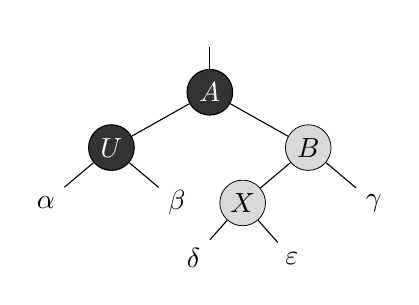
\begin{tikzpicture}[level/.style={sibling distance = 5cm/#1, level distance = 2em}] 
  \node {}
  child{
    node [black_node] {$A$}
    child{ node [black_node] {$U$}
      child{ node {$\alpha$}}
      child{ node {$\beta$}}
		}
    child{ node [red_node] {$B$} 
      child{ node [red_node] {$X$}
        child{ node {$\delta$}}
        child{ node {$\varepsilon$}}
      } 
      child{ node {$\gamma$}}
    }
  }; 
\end{tikzpicture}
\end{center}

  {\scriptsize
    a) the parent $B$ of $X$ is red, the uncle of $X$ is black, $B$ is the right
    child of its parent and $X$ is the left child of $B$
  }

  \columnbreak

\begin{center}
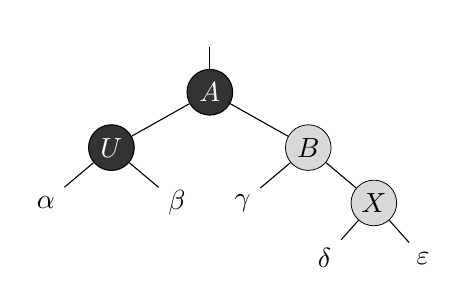
\begin{tikzpicture}[level/.style={sibling distance = 5cm/#1, level distance = 2em}] 
  \node {}
  child{
    node [black_node] {$A$}
    child{ node [black_node] {$U$}
      child{ node {$\alpha$}}
      child{ node {$\beta$}}
		}
    child{ node [red_node] {$B$} 
      child{ node {$\gamma$}}
      child{ node [red_node] {$X$}
        child{ node {$\delta$}}
        child{ node {$\varepsilon$}}
      } 
    }
  }; 
\end{tikzpicture}
\end{center}

  {\scriptsize
    b) the parent $B$ of $X$ is red, the uncle of $X$ is black, $B$ is the right
    child of its parent and $X$ is the right child of $B$
  }
\end{multicols} 

% Described cases occurs with some sub-tree after some number of insert/delete
% operations. Before inserting node $X$ this sub-tree should satisfied (by
% construction) properties of RB trees:

A red-black tree is a binary tree that satisfies the following \textbf{red-black
  properties} \cite[13.1]{introtoalg}: 

\begin{enumerate}
\item Every node is either red or black.
\item The root is black.
\item Every leaf (NIL) is black.
\item If a node is red, then both its children are black.
\item For each node, all simple paths from the node to descendant leaves contain the
same number of black nodes. 
\end{enumerate}

\textbf{In this cases property 4 is violated.}

For fix-up this cases, we use next algorithm \cite[p.320]{introtoalg}:\\

In case $( a )$, node is a left child of its parent. We immediately use a
right rotation to transform the situation into case $( b )$, in which node is a
right child. Because both $X$ and its parent $B$ are red, the rotation affects
neither the black-height of nodes nor property 5.\\

In case $( b )$, we execute some color changes and a left rotation, which
preserve property 5, and then, since we no longer have two red nodes in a row,
we are done. 

\begin{center}
  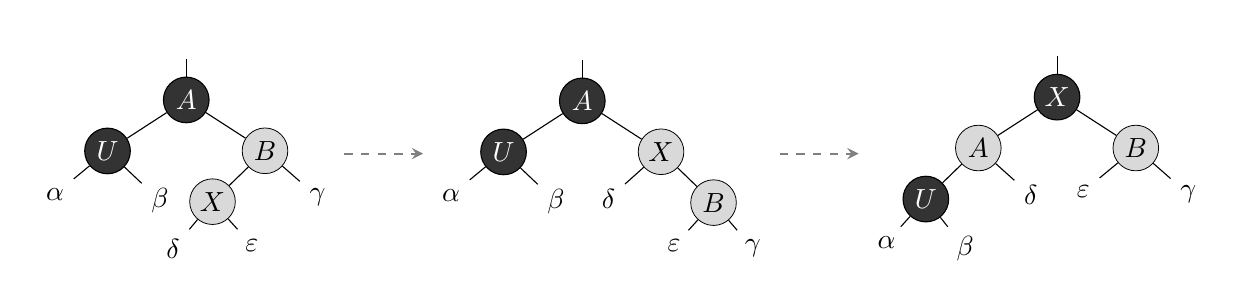
\begin{tikzpicture}[
    >=stealth,
    every node/.style={anchor=north},
    level/.style={sibling distance = 4cm/#1, level distance = 1em}
    ] 
  \node (case a) []{\tikz{%
    \node {}
    child{
      node [black_node] {$A$}
      child{ node [black_node] {$U$}
        child{ node {$\alpha$}}
        child{ node {$\beta$}}
      }
      child{ node [red_node] {$B$} 
        child{ node [red_node] {$X$}
          child{ node {$\delta$}}
          child{ node {$\varepsilon$}}
        } 
        child{ node {$\gamma$}}
      }
    };
  }}; 
  \node(case b)[right=of case a]{\tikz{%
    \node {}
    child{ node [black_node] {$A$}
      child{ node [black_node] {$U$}
        child{ node {$\alpha$}}
        child{ node {$\beta$}}
      }
      child{ node [red_node] {$X$} 
        child{ node {$\delta$}}
        child{ node [red_node] {$B$}
          child{ node {$\varepsilon$}}
          child{ node {$\gamma$}}
        } 
      }
    };
  }}; 
  \node(case c)[right=of case b]{\tikz{%
    \node {}
    child{ node [black_node] {$X$}
      child{ node [red_node] {$A$}
        child{ node [black_node] {$U$}
          child{ node {$\alpha$}}
          child{ node {$\beta$}}
        }
        child{ node {$\delta$}}
      }
      child{ node [red_node] {$B$} 
        child{ node {$\varepsilon$}}
        child{ node {$\gamma$}}
      }
    };
  }}; 
  \draw [->, dashed, thick, black!50] (case a) edge (case b);
  \draw [->, dashed, thick, black!50] (case b) edge (case c);
\end{tikzpicture}
\end{center}

\textit{Each of the sub-trees $\gamma$, $\varepsilon$, $\delta$, has a black
  root from property 4 and each has the same black-height the same as uncle sub-tree.}

\section{Knuth-Morris-Pratt algorithm}

\begin{theorem}
  $p$ is a period of $T \text{, iff } (T[i - p] = T[i + p])$, where $i \in [1+p \dots n-p]$
\end{theorem}

\textit{\color{Gray} As you can see, I changed little bit statement, to deal
  with boundaries}

\begin{proof}
  Lets consider graphical representation of period:\\

  This is representation of same string $T$, but with different shifts.

  First one without shift, second with shift $p$, third with shift $2p$.
  
\begin{center}
 \begin{tikzpicture}
    [
      >=stealth,
      bar/.style = {rectangle, draw, minimum height=0.2cm, minimum width=2cm},
      even/.style = {fill=gray!30},
      odd/.style = {fill=black!60}
    ]
    \begin{scope}[shift={(1cm,0)}]
      \draw [gray!50,step=2cm,dashed] (-4,-1.9) grid (7.9,1.9);
    \end{scope}

    \node at (-2,1) [bar, even] (o0) {};
    \node at (0,1) [bar, odd] (o1) {};
    \node at (2,1) [bar, even] (o2) {};
    \node at (4,1) [bar, odd] (o3) {};
    \node at (6,1) [bar, even] (o4) {};
    \node at (8,1) [bar, odd, dotted, path fading=last] (o5) {};

    \node at (0,0) [bar, even] (t1) {};
    \node at (2,0) [bar, odd] (t2) {};
    \node at (4,0) [bar, even] (t3) {};
    \node at (6,0) [bar, odd] (t4) {};
    \node at (8,0) [bar, even, dotted, path fading=last] (t5) {};

    \node at (2,-1) [bar, even] (p1) {};
    \node at (4,-1) [bar, odd] (p2) {};
    \node at (6,-1) [bar, even] (p3) {};
    \node at (8,-1) [bar, odd, dotted, path fading=last] (p4) {};

    \draw [->, thin] (-3,0)--(-1,0);
    \node at (-2, -0.2) {$p$};
    \draw [->, thin] (-3,-1)--(1,-1);
    \node at (-2, -1.2) {$2p$};

    \foreach \x/\alp in {-2/$s_1$,0/$s_2$,2/$s_3$,4/$s_4$,6/$\dots$,8/$s_{k}$}{
      \node at (\x,0.5) {\small \alp};
    }

    \foreach \x/\alp in {0/$s_1$,2/$s_2$,4/$s_3$,6/$\dots$,8/$s_{k+1}$}{
      \node at (\x,-0.5) {\small \alp};
    }

    \foreach \x/\alp in {2/$s_1$,4/$s_2$,6/$\dots$,8/$s_{k+2}$}{
      \node at (\x,-1.5) {\small \alp};
    }

\end{tikzpicture}\\
\textit{\color{Gray}Coloring doesn't represent difference, but just for visual separation}\\
\end{center}

String T could be represent as concatenation of their sub-strings
$s_1 \cdot s_2 \cdot ... \cdot s_n$\\

By definition of period $p$:

\begin{equation}
T[i] = T[i+p] \text{, where } i \in [1 \dots n-p]
\end{equation}

Thus, 
$s_2 \cdot s_3 \cdot ... \cdot s_n = s_1 \cdot s_2 \cdot ... \cdot s_{n-1}$, and
$s_1 = s_2 = ... = s_n$

This means that if string $T$, we could represent as $T = s \cdot s \cdot ...
\cdot s$, then:

\begin{equation}
  T=s \cdot s \cdot ... \cdot s \implies p = k|s|
  \footnote{As soon as multiple shift will give same position in sub-strings and equation (1) is true}
  \text{, where } k \in N
\end{equation}

Thus we could generalize equation (1) and (2) as:
 
\begin{equation}
  p_{min} = |s_{min}| \implies T[i] = T[i + kp_{min}]
\end{equation}

where
$p_{min}$ is a minimal period,
$s_{min}$ - minimal sub-string and $k \in N$.

We could replace the variable $i = j - p_{min}$,
then for particular case $k=2$ equation (3) takes the form:

\begin{equation}
  p_{min} = |s_{min}| \implies T[j-p_{min}]=T[j+p_{min}]
\end{equation}

Lets consider string period definition from other hand:

\begin{equation}
  T[i] = T[i + p] \implies p \text{ - period}
\end{equation}

We could symmetrically apply transformations described above, and get:

\begin{equation}
  T[j-p_{min}]=T[j+p_{min}] \implies p_{min} = |s_{min}| 
\end{equation}

Finally from (4) and (6):

$$ p \text{ - period} \iff T[j-p_{min}]=T[j+p_{min}] $$
\end{proof}


\paragraph{To compute the minimal period of the string}
we could use the Knuth-Morris-Pratt algorithm. More precisely we should
use prefix function $\pi$ described in book\cite[p.1003]{introtoalg}. \\

That is, $\pi[q]$ is the length of the longest prefix of $T$ that is a proper
suffix of $T_q$. Thus (in case $q = T.length$) we could calculate period as:\\

$$ p_{min} = T.length - \pi[T.length] $$

\section{Suffix array}

The occurrence of pattern $P$ in string $T$, correspond to interval $[L_p, R_p]$
in the suffix array for $T$. As soon as all suffixes of a string sorted
lexicographical, thus we can apply binary search to quickly locate occurrence of
pattern $P$ in a string, by comparison with each suffix of string.\\

The starting position $L_p$ of interval is a first suffix that greater than or
equals to pattern lexicographical. The ending position $R_p$ is a first suffix,
which sub-string of length $|P|$, lexicographical greater than pattern. This
definition of right boundary of the interval is fuzzy, but it important to
mention that we will compare only prefixes of suffixes to find it.\\

\IncMargin{1em}
\begin{algorithm}[H]
  \SetAlgoNoEnd\SetAlgoNoLine
  \SetNlSkip{1.5em}
  \DontPrintSemicolon

  \nonl \textsc{Search-of-$R_p$}$(T, P, SA)$\;
  $l \leftarrow 0$\;
  $r \leftarrow $ \textsc{SA.Length}{\color{Gray}\tcp*{ or \textsc{T.Length + 1}}}
  $q \leftarrow $ \textsc{P.Length}\;

  \While {$l < r$}{
    $m \leftarrow \lfloor (l+r)/2 \rfloor$\;
    \eIf{$P \geq _{lex} T[SA[m] \dots SA[m]+q] $}{
      $l \leftarrow m + 1$
    }{
      $r \leftarrow m $
    }
  }
  \Return $R_p \leftarrow m$
\end{algorithm}

Obviously we could compare $SA[1]$ and $SA[m]$ for handling absence of matching
before search (some kind of first looking), but this is premature optimization.\\

At line 6 we compare prefix of suffix with pattern. Whole while loop ends when
$l$ and $r$ positions converge and finally function yields position of first
suffix which prefix greater than or equal to pattern.\\

Then we could analyze compare with $L_p$. If they are the same - there is no
occurrence.\\

Also we should check boundary case when $R_p = m$, it could be false positive.

\bibliography{hw2}

\end{document}